\documentclass{standalone}
\usepackage[dvipsnames]{xcolor}
\usepackage{tikz}
\usetikzlibrary{arrows.meta, calc, positioning, shapes.geometric}

\tikzset{%
  every path/.style={thick},
    edge/.style={%
        ->,
        >={Stealth[scale=1]},
    },
    usercode/.style={%
        rectangle,
        fill=orange!80,
        draw=black, thick,
        minimum width=3em,
        rounded corners=2pt,
        text=white,
        font=\footnotesize,
        text centered,
    },
    lib/.style={%
        ellipse,
        fill=blue!80,
        minimum width=.12\linewidth,
        minimum height=.04\linewidth,
        rounded corners=2pt,
        text=white,
        font=\footnotesize,
        text centered,
    },
    solver/.style={%
        rectangle,
        fill=Green,
        draw=black, thick, dashed,
        text=white,
        font=\footnotesize,
        text centered,
        minimum width=3em,
        rounded corners=2pt,
    },
}

\begin{document}
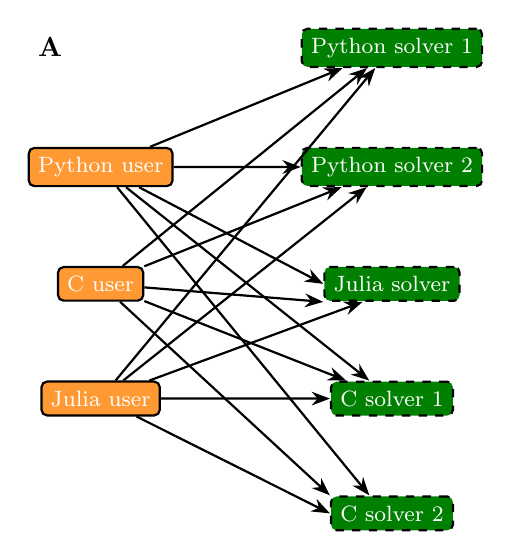
\begin{tikzpicture}
	\coordinate (left_side) at (-1.7, 0);
	\coordinate (right_side) at (2, 0.0);

	\node [usercode,] at (left_side) (user_c) {C user};
	\node [usercode, above=of user_c] (user_py) {Python user};
	\node [usercode, below=of user_c] (user_jl) {Julia user};

	\node [solver,] at (right_side) (solver1) {Julia solver};
	\node [solver, above=of solver1] (solver2) {Python solver 2};
	\node [solver, above=of solver2] (solver3) {Python solver 1};
	\node [solver, below=of solver1] (solver4) {C solver 1};
	\node [solver, below=of solver4] (solver5) {C solver 2};

	\node at (current bounding box.north west) [anchor=north west] {\textbf{A}};

	\draw[edge] (user_py) -- (solver1.west);
	\draw[edge] (user_py) -- (solver2);
	\draw[edge] (user_py) -- (solver3);
	\draw[edge] (user_py) -- (solver4);
	\draw[edge] (user_py) -- ($(solver5.north west) + (0.5, 0)$);

	\draw[edge] (user_c) -- (solver1.south west);
	\draw[edge] (user_c) -- (solver2);
	\draw[edge] (user_c) -- (solver3);
	\draw[edge] (user_c) -- (solver4);
	\draw[edge] (user_c) -- (solver5.north west);

	\draw[edge] (user_jl) -- ($(solver1.south west) + (0.5, 0)$);
	\draw[edge] (user_jl) -- (solver2);
	\draw[edge] (user_jl) -- (solver3);
	\draw[edge] (user_jl) -- (solver4);
	\draw[edge] (user_jl) -- (solver5.west);
\end{tikzpicture}
\end{document}
